
% !TEX encoding = UTF-8 Unicode

\documentclass[a4paper]{article}

\usepackage{color}
\usepackage{url}
\usepackage[T2A]{fontenc} % enable Cyrillic fonts
\usepackage[utf8]{inputenc} % make weird characters work
\usepackage{graphicx}
\usepackage{float}

\usepackage[english,serbian]{babel}
%\usepackage[english,serbianc]{babel} %ukljuciti babel sa ovim opcijama, umesto gornjim, ukoliko se koristi cirilica

\usepackage[unicode]{hyperref}
\hypersetup{colorlinks,citecolor=green,filecolor=green,linkcolor=blue,urlcolor=blue}

%\newtheorem{primer}{Пример}[section] %ćirilični primer
\newtheorem{primer}{Primer}[section]

\begin{document}

\title{Pregled razvoja računarstva u 21. veku\\ \small{Seminarski rad u okviru kursa\\Računarstvo i društvo\\ Matematički fakultet}}

\author{Jana Milutinović 448/2022\\ janamltnvc@gmail.com}
\date{}
\maketitle

\abstract{
Svedoci smo, a i učesnici tehnološke revolucije koja je iz korena promenila svet u kome živimo. Digitalna pismenost je postala ključna profesionalna veština svakog radno sposobnog čoveka.
U ovom radu se istražuje šta je prethodilo ekspanziji računarstva u vremenu u kom 
živimo, kako je tekao napredak i razvoj tehnologija bez kojih danas ne možemo, do čega nas je tehnologija dovela i kako utiče na naš svakodnevni život.


\tableofcontents



\newpage

\setlength{\parskip}{1em}


\section{Uvod}
\label{sec:uvod}

Istorija računarstva seže daleko unazad, čak do antičkih civilizacija koje su koristile abakus za osnovne računske operacije. Tokom vremena, razvijali su se mehanički digitroni za rad sa dekadnim i binarnim brojevnim sistemima. Početkom 19. veka, konstruisane su prve programabilne mašine, uključujući čuvenu analitičku mašinu koja je omogućila programiranje putem bušenih kartica, uz pionirske napore Ade Bajron i Čarlsa Bebidža.

U 20. veku, računarstvo je doživelo značajne prekretnice. Pojavili su se prvi elektronski računari, uključujući ENIAC, prvi računar opšte namene. Ova era obeležena je i pojavom osnovnih koncepata, kao što su fon Nojmanova arhitektura i koncept elektronskog memorisanja.

Uz računare, mnogi ključni koncepti računarstva su teoretski osmišljeni tokom prethodnog veka, ali su se praktično razvijali tek u poslednjih nekoliko decenija. Umrežavanje računara putem WAN mreža počelo je 60-ih godina, a internet i World Wide Web (WWW) su omogućili globalno povezivanje računara tokom devedesetih. Jezici višeg nivoa, kao što su FORTRAN, COBOL, Algol i LISP, datiraju iz pedesetih i šezdesetih godina 20. veka. Koncepti kao mašinsko učenje i neuronske mreže imaju dugu istoriju, ali su zahtevali vreme i tehnološki napredak kako bi postali praktično primenjivi.

U ovom radu se analiziraju najznačajnija tehnološka dostignuća 21. veka i istražuje kako su aktuelne teme oblikovale našu tehnološku budućnost.

\setlength{\parskip}{1em}

\section{Napredak računarstva u 21. veku}
\label{sec:rac_21. vek}
Sa današnje tačke gledišta primećujemo nekoliko presudnih trenutaka koji su doprineli razvoju tehnologije kakvu danas koristimo. Ključni događaji bi bili popularizacija interneta i razvoj pametnih uređaja početkom 21. veka a kasnije i razvoj društvenih mreža, veštačke inteligencije, Cloud i blockchain tehnologija, Interneta pametnih uređaja. 
\subsection{Internet}
WWW i internet su se pojavili još početkom 1990-ih, ali tek početkom 2000-ih godina WWW postaje mainstream, tj. široko rasprostranjen. U 2000. godini na internetu postoji oko 361 milion korisnika (oko 5\% svetske populacije), a već 2005. taj broj je skočio na oko 1 milijardu 18 miliona. Danas je skoro 70\% čitave populacije na mreži \cite{worldstats}. Veliki broj korisnika interneta dovelo je do velike količine dostupnih korisničkih podataka, pa su razvijani mnogi algoritmi, alati i koncepti za razne vrste obrade tih podataka, što je dovelo do napretka i razvoja najvažnijih polja modernog računarstva. Kao što znamo mnogi koncepti mašinskog učenja i veštačke inteligencije se zasnivaju na modelovanju velike količine podataka, predikciji na osnovu poznatih informacija i dr.
Danas se veliki obim poslovanja izvršava u internet okruženju a domen korišćenja računara je veoma širok.
\subsection{Vremenska linija}

U nastavku je prikazana vremenska linija 21. veka sa važnim dostignućima u računarskoj nauci i tehnologiji generalno. 


\begin{figure}[h!]
\begin{center}
\includegraphics[width=15cm]{Timeline Cycle Visual Charts Presentation in Blue White Teal Simple Style.jpg}
\end{center}
\caption{Prva dekada}
\label{fig:kvant}
\end{figure}
\begin{figure}[h!]
\begin{center}
\includegraphics[width=15cm]{4.jpg}
\end{center}
\caption{Druga dekada}
\label{fig:kvant}
\end{figure}


Početkom dvehiljaditih se pojavljuje prvi mobilni telefon sa kamerom, USB disk, a kompanija Honda predstavlja prvog čovekolikog robota. Zatim pratimo razvoj operativnih sistema koje danas koristimo - MAC OS X i Windows XP, zatim razvoj dobro poznatih društvenih mreža 2003-2004. Ubrzo nakon formiranja Laboratorije za Kompjutersku nauku i veštačku inteligenciju na MIT Univerzitetu, autonomno vozilo kreirano na Stenford Univerzitetu pobedjuje veliku automobilsku trku. Autonomna vožnja je i danas ključan pojam i važna oblast veštačke inteligencije koja se rapidno razvija i na kojoj se intenzivno radi jos od početka veka. Još 2006. godine se uvodi pojam Cloud-a, iako tek u poslednjoj dekadi intenzivno pričamo o ovoj temi i prebacujemo se na ovu tehnologiju. 2007. je zanimljiva godina kada se pojavljuju Kindl i prvi Iphone, dok se paralelno bavimo prostorom, kako fizičkim tako i ovim na cloud-u, pa tako se pojavljuje prvi hard disk sa memorijom od 1 TB, ali je pokrenut i DropBox - online skladište. 2009. je razvijen BitCoin a tek od 2018. godine je primena Blockchain tehnologije proširena i na druge industrije. Poslednje godine vezane su uglavnom za ekspanziju svih podgrana veštačke inteligencije - robotike i razvoja veštačkih organa, robota koji se koriste u razne svrhe, autopilota i trenutno najpopularnijeg veštačkog pomoćnika - ChatGPT.

\setlength{\parskip}{1em}


% \begin{center}
% 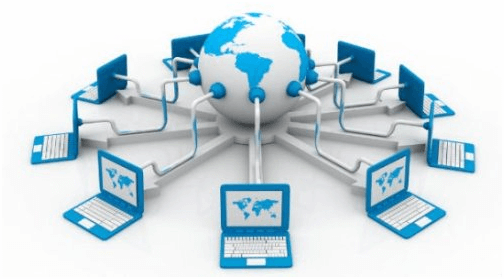
\includegraphics[scale=0.4]{world-wide-web.png}
% \end{center}
% \caption{Slika 1: World Wide Web}
% \label{world wide web}

\subsection{Društvene mreže}
{\bf Pojava društvenih mreža} kao glavnog medijuma komunikacije danas je dovela do velikih promena u poslovnom svetu, u marketingu, internet kupovini, oglašavanju, pa je shodno tome bilo potrebno razviti jezike, baze podataka i ostale koncepte i prilagoditi ih korišćenju na internetu. 

\subsection{Mobilno računarstvo}
Razvoj hardvera, kao na primer mobilnih telefona početkom dvehiljaditih je jedan od ključnih perioda u savremenoj istoriji.
{\bf Razvoj mobilnog računarstva} je jedan od najvećih dostignuća 21. veka. Razvoj pametnih telefona je bio revolucionaran način na koji ljudi komuniciraju sa tehnologijom i međusobno, na bilo kojoj udaljenosti.  Mobilni telefoni su omogućili ljudima da se brzo i jednostavno povežu na internet i da pristupaju informacijama i uslugama u realnom vremenu i u pokretu, a naravno i da se relativno jeftino povežu sa ljudima na udaljenim lokacijama. 
Razvoj mobilnog računarstva imao je dubok uticaj na mnoge industrije, uključujući maloprodaju, zabavu i društvene medije, zdravlje, turizam, kretanje. Mobilne aplikacije postale su glavni način za kompanije da dođu do potrošača, a ekonomija aplikacija je brzo rasla.
Ovaj trenutak morao je da isprati i softverski napredak, pa se tako dešava i ekspanzija razvoja novih tehnologija za mobilne uređaje, kao što su programski jezici Kotlin i Swift, mobilno plaćanje, usluge zasnovane na trenutnoj lokaciji poput navigacionih aplikacija, praćenja vozila i dostava, servisa za retragu restorana i prodavnica i drugo. 

\subsection{Veštačka inteligencija}
{\bf Razvoj veštačke inteligencije}
Veštačka inteligencija doživljava svoju ekspanziju usled iznenadne dostupnosti masivnih skupova korisničkih podataka, pa mašinsko učenje postaje "vruća tema" računarstva
jer je shvaćeno da veb podaci mogu hraniti takve algoritme. Početkom dvehiljaditih godina razvoj veštačke inteligencije doživljava ubrzan napredak kada je računar pobedio svetskog velemajsotra u šahu i dokazao teoreme koje čovek dugo nije uspevao da dokaže. 
Osim pomenutog, javio se i talas vrlo uspešnih sistema zasnovanih na \„dubokom učenju\“ – sistema koji su uspešno vršili prepoznavanje lica na fotografijama, prevođenje prirodnih jezika, navigaciju vozila i drugo. Veštačka inteligencija danas je skoro sveprisutna, a opšte je uverenje da će se ta sveprisutnost u budućnosti dalje proširivati i produbljivati \cite{vi}.

Od 2010. godine počinje era veštačke inteligencije koja i dalje traje. Moćni računari novih generacija omogućili su realizaciju i impementaciju neuronskih mreža koje su teorijski razvijene jos 1950-ih.
Kroz duboko učenje ostvarili su se fantastični rezultati u mnogim poljima, kao što su računarski vid, automatsko prevođenje, igranje strateških igara, itd. Ovi rezultati zasnovani su na statistici i mašinskom ucenju.

\subsubsection{Veštačka inteligencija danas - filozofija, budućnost, etika}
Cilj veštačke inteligencije je {\bf oponašanje prirodne inteligencije } - znanje i zaključivanje na osnovu datih informacija, potvrđenih činjenica ali i hipoteza  i nepotpunih informacija, usvajanje novih znanja i sposobnost komunikacija sa drugim inteligentnim bićima ili mašinama. Zato je bitan { \bf kvalitet baze znanja } - koji su izvori podataka, koliko su isti tačni i provereni, da li su podaci sa interneta, posebno sa društvenih mreža filtrirani i provereni.

Zato se i javljaju brojna opšta i etička pitanja, kao na primer, da li su sloboda govora i mišljenja prednost ili mana ovakih sistema? 
Sa jedne strane, računaru je potrebno što više informacija kako bi sam doneo odluku, ali će nepogodne informacije dovesti do loših, možda i fatalnih rezultata i ishoda. 

Teško je postaviti granicu između ljudske i veštačke inteligencije. Za sada ne postoji telo koje može tu granicu da postavi a još uvek to verovatno nije ni moguće. Da li mašine treba samostalno da donose sve odluke?  Da li je strah od "mašina koje misle" opravdan? Da li autonomno vozilo u potpunosti sme da preplavi naše puteve? samo su neka od pitanja na koja se trudimo da odgovaramo svakog dana ali i dalje nismo blizu tačnog odgovora.

Trenutno su sve velike kompanije uključene u neki vid razvoja virtualnog asistenta-chat bot-a i deluje da je to tema koja će biti aktuelna u narednih par godina jer se pokazalo da se VI jako efikasno može koristiti za automatizaciju mnogih zadataka vezanih za obradu teksta, slika i multimedija. 


\setlength{\parskip}{1em}


\subsection{Kvantni računari}	
{\bf Kvantni računar} je zamišljen kao mašina koja koristi koncepte kvante mehanike kako bi rešila neki problem brže nego što je to moguće na klasičnim računarima. Dok klasični računar reprezentuju bitovi, kvantni
reprezentuju kjubiti (qbit). {\bf Kjubit} osim nule i jedinice ima i jedno dodatno stanje - superpoziciju - koja omogućava paralelizaciju
izračunavanja i pretrage \cite{kvantni}.

Očekuje se da bi moć ovih računara bila u njihovoj sposobnosti da izvršavaju brzu pretragu i obrađuju i čuvaju ogromnu količinu podataka, učeći iz prethodnih zadataka i efikasno rešavajući različite probleme. Smatra se da će zbog ovih mogućnosti u budućnosti biti od velike pomoći u pronalaženju novih lekova, u borbi protiv klimatskih promena, poboljšavanju robotike i celokupnom olakšavanju svakodnevnog života.

Tehnologija će morati da evoluira u kvantno otporan sistem u narednoj deceniji. Ovo prvenstveno važi zato što bi kvantni računari potencijalno mogli postati toliko moćni da napadnu kriptovalute i razbiju blockchain. Generalno javio bi se {\bf problem dekriptografije} jer bi za probijanje bilo koje
kriptovane šifre super računaru trebale bi godine rada
a kvantnom, zbog paralelizma u obradi, nekoliko
sekundi.  Bilo bi potrebno razviti sve nove sisteme zaštite.
Takođe, očekuje se da bi ovakve mašine mogle da reše {\bf problem optimizacije  }-
obilasci gradova, problem najkraćeg puta, kao i {\bf problem pretraživanja} velike količine podataka. 

\begin{figure}[h!]
\begin{center}
\includegraphics[scale=0.65]{kvantni.jpg}
\end{center}
\caption{Kvantni računar}
\label{fig:kvant}
\end{figure}

\setlength{\parskip}{1em}


\subsection{ Druge aktuelne teme 21. veka}	
Današnji programer ima širok spektar tehnologija i oblasti kojima može da se bavi. Neke od oblasti savremenog računarstva su:

		\begin{itemize}
		    \item Algoritmika 
\item Strukture podataka 
\item Programski jezici 
\item Operativni sistemi 
\item Istraživanje podataka 
\item \textbf{Veštačka inteligencija }
\item \textbf{Robotika} 
\item Računarska grafika 
\item Kriptografija 
\item\textbf{Kvantno računarstvo} 

		\end{itemize}
Sve podgrane veštačke inteligencije su definitivno te koje se najviše razvijaju i usavršavaju iz dana u dan i čija primena je najšira ali važno je i spomenuti koliko je razvoj Cloud tehnologija uticao na razvoj biznisa, deljenje podataka, skalabilnost generalno, na povećanje bezbednosti sistema i svih segmenata biznisa. Cloud infrastruktura je smanjila troškove i povećala fleksibilnost pri implementaciji.

Tema koja je vrlo aktuelna na svetskim IT konferencijama poslednjih godina je svakako i {\bf Internet of Things} - Internet pametnih uređaja. IOT je skup fizičkih uređaja koji su hradverski opremljeni tako da mogu biti povezani na internet, u svrhu deljenja i prikupljanja podataka. Ovime im se daje određena digitalna inteligencija, jer bez angažovanja čoveka koriste podatke i regulišu svoj rad. Ti uređaji mogu biti jednostavni poput igračaka za decu, kućnih aparata, satova ali i recimo mlazni motori, dronovi uz čiju pomoć može i da se kontroliše životna sredina, bezbednosni nadzor, pametno grjanje, osvetljenje i drugo, što je dovelo i do pojave pametnih kuća i gradova. Primena IOT-a je jako široka i može biti od velike koristi u poljoprivredi, medicini, privredi, saobraćaju. IOT će verovatno i u narednoj dekadi biti tema o kojoj se priča baš zbog velikih prednosti na razne socio-ekonomske grane \cite{iot}.

Tržište {\bf virutelne relanosti} je još jedna oblast u usponu zbog velike praktične primene u mnogim različitim oblastima. Zabava, turizam i virutelna putovanja, arhitektura u vidu vizualizacija projekata, virtuelna naselja, medicina, edukacija su samo od nekih najvažnijih oblasti u kojima VR ima primenu. Još sada se VR koristi kako bi se modeliralo ljudsko telo ili specifičan organ radi bolje vizualizacije i planiranja operacija. VR se koristi za učenje jezika, putovanja i drugo. 

\newpage
\section{Zaključak}
\label{Zaključak}

Neminovno je da živimo u eri svojevrsne informatičke revolucije, koliko god bili spremni da prihvatimo novine koje nam se plasiraju iz dana u dan. Pre samo 10ak godina nije bilo moguće zamisliti da ćemo danas plaćati putem telefona, da će Google prevodilac biti toliko napredan da se možemo potpuno sporazumeti sa osobama čiji jezik ne poznajemo, da ćemo koristiti alate koji rade umesto nas, da ćemo plaćati virtuelnim valutama, da će kamera na našem telefonu moći da prepoznaje lica, predele, dokumenta, da čita pisani tekst... 

Svaki pomalo nekontrolisani napredak ima svoje prednosti i mane, pa tako uz omasovljenost interneta i uz brz i lak pristup informacijama, sigurno imamo obaveštenije društvo, ali tačnost informacija je danas mnogo teže proveriti u nepreglednom moru istih. Danas uspevamo da rešimo kompleksne zadatke koje su decenijama bili zahtevni za tadašnju tehnologiju. Razvojem jedne nauke koja je postala implementirana u sve druge sigurno se doprinosi globalnom i generalnom razvoju opšteg znanja. Knjige i naučni članci su nam danas dostupni "na klik" . 
Sticanje znanja iz različitih obasti kroz online edukacije je jedan od velikih benefita za koji možemo biti zahvalni napretku tehnologije.  
Do početka dvehiljaditih bilo je teško povezati se sa ljudima i mašinama na udaljenim krajevima sveta, dok je danas globalno umrežavanje naša svakodnevica što nas čini stanovnicima celog sveta. Ništa više nam nije tako nedostupno i nepoznato, koliko god bilo udaljeno.


Nažalost, ovaj rapidni napredak nas je uhvatio i nespremne za neke nove probleme koji su se pojavili. Neželjenog sadržaja na internetu je mnogo i teško ga je ograničiti. Součavamo se sa brojnim posledicama prekomernog korišćenja pametnih uređaja koji utiču na psihofizički razvoj, akademske i druge performanse, lečimo se od socijalne distanciranosti i tehnološke anksioznosti \cite{techanx}. Svetska zdravstvena organizacija je uključila poremećaj igranja video igara u poslednju reviziju Međunarodne klasifikacije bolesti (ICD-11) kao ponašanje sa adiktivnim svojstvima \cite{gamingdisorder}. 
Učestvovanjem na online nebu potencijalno postajemo žrtve prevara, krađa i može nam biti ugrožena bezbednost. Tehnologija je i veliki zagađivač planete i negativno utiče na iscrpljivanje prirodnih resursa, zagađenje vazduha i nagomilavanje otpada, ali se tehnologija može i iskoristiti u borbi protiv zagađenja planete i ovo je takođe jedna od grana koja će se rapidno razvijati u narednim godinama \cite{pollution}.



U budućnosti, veštačka inteligencija će se razvijati u mnogim oblastima. Prvo, medicina će videti napredak kroz AI u dijagnostici, lečenju i personalizovanoj medicini. Drugo, sektor autonomnih vozila i transporta će i dalje rasti, uz sve sofisticiranije AI sisteme za sigurniju vožnju. Treće, AI će transformisati oblast obrazovanja putem personalizovane nastave i praćenja napretka učenika. Četvrto, u oblasti ekologije, AI će igrati ključnu ulogu u rešavanju problema klimatskih promena i upravljanju prirodnim resursima. Razvoj AI kroz ChatGPT u budućnosti će se usmeriti na sve dublje razumevanje i kontekstualno relevantne odgovore, pružajući korisnicima još naprednije i personalizovane interakcije.

Poslednji pasus generisan je od strane chatbot-a ChatGPT i to je njegovo viđenje budućnosti razvoja veštačke inteligencije. S obzirom da spomenuto realno i jesu aktuelne teme u računarstvu, očekivan je i njihov dalji razvoj i napredak. Ostaje da ispratimo da li nam se roboti razvijaju u pravom smeru, da li će veštačka prevazići prirodnu inteligenciju i kakav nam to novi svet donosi.

% \setlength{\parskip}{27em}

\addcontentsline{toc}{section}{}
\appendix  
%\bibliography{cites} 
\bibliographystyle{plain}

\begin{thebibliography}{Literatura}
    \bibitem{vi}
        \href{http://poincare.matf.bg.ac.rs/~janicic//books/VI_B5.pdf}{Veštačka inteligencija}{ Predrag Janičić, Mladen Nikolić, 2023.}

    \bibitem{kvantni} 
        \href{http://www.racunarstvo.matf.bg.ac.rs/MasterRadovi/2017_06_05_Nikola_Spasojevic/rad.pdf}{Implementacija nekih algoritama na kvantnim računarima} {Nikola Spasojević, 2019}

    \bibitem{worldstats}
        \href{https://www.internetworldstats.com/emarketing.htm}{Internet Growth statistics}

    \bibitem{p1}
        \href{http://poincare.matf.bg.ac.rs/~sana/Programiranje1_M/p1_I_smer.pdf}{Programiranje 1 kroz programski jezik C }{
Filip Marić, Predrag Janičić, Beograd, 2014.}

    \bibitem{ml}
        \href{https://ml.matf.bg.ac.rs/readings/ml.pdf}{Mašinsko učenje}{Mladen Nikolić, Anđelka Zečević, Beograd, 2019.}

    \bibitem{timeline}
        \href{https://www.computerhistory.org/timeline/}{Timeline of Computer History}

    \bibitem{21st}
        \href{https://academicinfluence.com/inflection/study-guides/computer-science-2000-2020}{A Brief History of Computer Science: 2000-2020}
        
    \bibitem{istfil}
        \href{https://stasa.in.rs/wp-content/uploads/IFR-04.pdf}{Istorija i filozofija
računarstva}{Staša Vujičić Stanković}
    \bibitem{techanx}
        \href{https://files.eric.ed.gov/fulltext/ED501623.pdf}{Factors Influencing Computer Anxiety and Its Impact on E-Learning Effectiveness: A
Review of Literature }

    \bibitem{pollution}
        \href{http://ijesi.org/papers/Conf.1802(ICMEEP)/Vol-5/12.%2053-55.pdf}{Impact of Technology on Environment}

    \bibitem{gamingdisorder}
        \href{https://www.who.int/news/item/14-09-2018-inclusion-of-gaming-disorder-in-icd-11}{Inclusion of “gaming disorder”}

    \bibitem{iot}
        \href{https://samoobrazovanje.rs/sta-je-internet-of-things-internet-inteligentnih-uredjaja/}{IOT osnove}
\end{thebibliography}
\newpage

\appendix
\section{ChatGPT}

ChatGPT je veštačka inteligencija ili jezički model koji je treniran na ogromnom korpusu tekstualnih podataka kako bi naučio razumevanje prirodnog jezika i generisanje tekstualnih odgovora na osnovu zadatih ulaza. Može se koristiti za različite svrhe, uključujući odgovaranje na pitanja, pružanje informacija, pomoć u rešavanju problema, generisanje sadržaja, davanje saveta i još mnogo toga. ChatGPT može komunicirati na različitim jezicima i prilagoditi se različitim kontekstima. 

Kako sam kaže, važno je napomenuti da ChatGPT koristi tekstualnu obradu i generaciju na osnovu prethodnih tekstualnih ulaza, te da nema stvarnu svest ili razumevanje. Osim toga, njegovi odgovori se generišu na osnovu obimnog trening skupa podataka, ali se ne oslanja na aktuelne informacije nakon datuma svog poslednjeg ažuriranja, koji je septembar 2021. godine.

Chat GPT je alat koji ima široku primenu a jedna od glavnih prednosti bi bilo skraćivanje vremena pretrage i analize teme koju izučavamo, s obzirom da je model istreniran na velikoj količini podataka iz različitih izvora. Izučavajući temu seminarskog rada potrošila sam veći deo vremena na prikupljanje podataka i zaključivanje šta je to što se najčešće spominje, šta je najvažnija nit i na proveru informacija. Nakon nekoliko dana rada na prezentaciji na temu "Pregled razvoja računarstva u 21. veku", pitala sam ChatGPT da mi napravi prezentaciju na istu temu i ovo je bio njegov odgovor:

\begin{figure}[H]
% \begin{center}
\includegraphics[scale=0.65]{Merged_document.png}
% \end{center}
\caption{ChatGPT}
\label{fig:kvant}
\end{figure}

Može se uočiti velika sličnost između tema obrađenih u mom radu i onih koje je predložio ChatGPT. To mi je dalo potvrdu da je analiza urađena dobro i da su u radu pokrivene sve važne teme, ali je potrošeno mnogo sati na pronalaženje i isčitavanje svih relevantnih izvora. Zaključuje se da se ChatGPT može koristiti kao pomoć pri pisanju radova jer umnogome smanjuje vreme potrošeno na samu pripremu. Samoistraživanje je važno jer daje širu sliku izučavane teme a ne samo presek najvažnijih činjenica koje pruža ChatGPT. Za potpuno razumevanje oblasti koju izučavamo nije dovoljno da se oslanjamo na činjenice pružene od strane ChatGPT-a već je on pomoćno sredstvo koje nas može upoznati sa nekom temom, tako što će napraviti kostur osnovnih informacija i tema koje se dalje moraju produbiti. 

Iako je moćan u automatizaciji zadataka koji nam oduzimaju mnogo vremena, korišćenje ChatGPT-a mora biti kontrolisano i dobijene informacije se moraju uzimati sa rezervom. Postavlja se i pitanje etike korišćenja alata, jer kao što smo videli može generisati tekst na zadatu temu, koji korisnik može dalje plasirati kao svoj. ChatGPT može nam dati uvid na razne teme ali ima svoja ograničenja i ne može dati odgovor na sva pitanja. Kako sam kaže, ažuriran je u septembru 2022. godine i ne može nam dati aktuelne informacije. Ovo sam proverila i ChatGPT ne daje informacije o aktuelnim temama iz 2023. godine. Ukoliko model nije istreniran na neku temu, neće nam dati tačne informacije ili neće imati odgovor. Navodi da nije sposoban za obradu osetljivih informacija kao što su lični, finansijski i zdravstveni podaci. Ne bi trebalo da daje nelegalne i etički neprihvatljive savete i širenje mržnje. Nema sposobnost predviđanja budućnosti i da rešava komplekse kreativne zadatke. Na primer, ChatGPT nije znao ko su pojedini dugogodišnji profesori Matematičkog fakulteta ali je imao informacije o većini javnih ličnosti naše zemlje.
Deluje da model ne prihvata ispravke niti uči na osnovu informacija koje mi njemu pružamo. Na primer, model nema informacije o našoj poznatoj atletičarki Ivani Vuleta, ali zna ko je Ivana Španović. Iako se radi o istoj osobi koja je udajom promenila prezime, model ne prihvata moj komentar da je u pitanju ista osoba i na ponovni upit o tome ko je Ivana Vuleta dobijam odgovor da model nema informacija o osobi sa tim imenom. 

Pokušala sam da pitam ChatGPT kako se oseća osoba sa određenim emocionalnim i fizičkim simptomima. Modelu je postavljeno pitanje kako se oseća osoba koja ne govori puno, ima zabrinut pogled, podočnjake i plače i dobijen je vrlo detaljan odgovor o tome da opisano ukazuje na neko emocionalno opterećenje, uz potencijalna stanja u kojima se osoba nalazi i načine na koje možemo da pomognemo osobi koja je u tom stanju. Model ispravno prepoznaje znake raznih stanja kao što su zaljubljenost, potištenost, sreća, tuga, ushićenost, ponos i drugo a ono što je zanimljivo je da uvek navede da on ne može da čita osećanja drugih ljudi i da ako želimo da budemo sigurni, moramo pitati i razgovarati sa osobom kako bismo bili sigurni kako se oseća. 

Evo šta ChatGPT zaključuje sam o sebi:

"ChatGPT predstavlja impresivan napredak u oblasti prirodne jezičke obrade i komunikacije između ljudi i računara. ChatGPT ima potencijal da poboljša korisničko iskustvo u različitim oblastima, uključujući online podršku, automatizovanu asistenciju i generisanje sadržaja. Međutim, važno je uzeti u obzir i ograničenja modela, kao što su povremeni nepravilni odgovori i potreba za pažljivim praćenjem kako bi se osigurala tačnost informacija. U budućnosti, dalje fine-tjuningovanje i razvoj modela kao što je ChatGPT će verovatno unaprediti sposobnosti konverzacijskih AI sistema i omogućiti njihovu širu primenu u svakodnevnom životu."


\end{document}
